\documentclass[main]{subfiles}

\begin{document}

\chapter{Estimación del estado}

Como se deduce en el capítulo \ref{chap:modelo} el vector de estados es: $$X=\left\lbrace  x,y,z, \theta,\varphi,\psi, v_{q_z},v_{q_y},v_{q_z},\omega_{q_x},\omega_{q_y},\omega_{q_z} \right\rbrace$$.

Con el objetivo de agregar robustez a las medidas arrojadas por los sensores, se debe implementar algún algoritmo de estimación de estados que, corriendo en tiempo real, mantenga una estimación del estado mejor que la que se obtendría utilizando las medidas de los sensores.\\

El filtro de Kalman es un algoritmo que usa una serie de medidas ruidosas observadas a lo largo del tiempo y produce una estimación de alguna variable desconocida que resulta ser más precisa que la observación llana de la medidas. El filtro de Kalman opera recursivamente sobre el flujo de la entrada ruidosa y arroja la estimación estadísticamente óptima del estado.

Consiste básicamente en 2 etapas:\\
\begin{itemize}
  \item Predicción
  \item Actualización
\end{itemize}

En la figura \ref{fig:kal} se muestra un diagrama de flujo de la operación de un filtro de Kalman. Se parte de una estimación a priori del estado, la cual es utilizada como semilla para las posteriores iteraciones del filtro. En la etapa de \textbf{predicción}, el filtro produce una estimación del estado de las variables, junto con sus incertidumbres. Se hallan las variables $P_{k|k-1}$ y $\hat{x}_{k|k-1}$, correspondientes a la predicción de la matriz de covarianza estimada y la predicción del estado estimado, respectivamente. La covarianza, en la teoría de la probabilidad, es una medida de cuán juntas cambian 2 variables aleatorias. Si presentan un comportamiento similar tendrán una covarianza elevada y positiva, si el comportamiento es opuesto la covarianza será negativa y elevada en valor absoluto. Si las variables aleatorias no presentan relación, la covarianza será 0. Es una magnitud que no es sencilla de interpretar pero cobra vital importancia a la hora de entender el comportamiento del filtro.

\begin{figure}[h!]
	\centering
	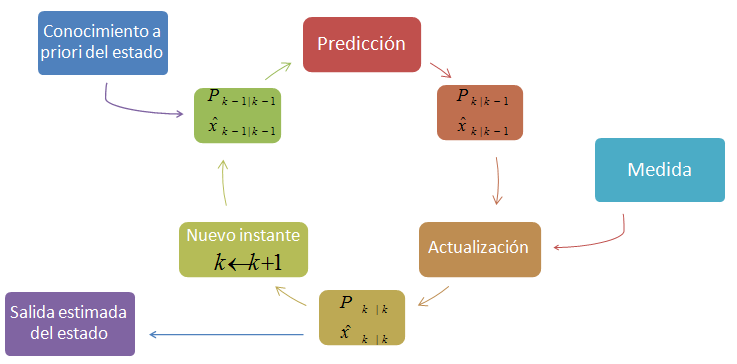
\includegraphics[width=.8\textwidth]{./pics_kalman/kal.png}
	\caption{Diagrama de flujo del filtro de Kalman}
	\label{fig:kal}
\end{figure}

Una vez que llega la siguiente medida de los sensores, contaminada necesariamente con ruido, las estimaciones son actualizadas en la etapa de \textbf{actualización}, mediante la utilización de un \emph{promedio ponderado}, dándole mayor peso a las estimaciones con menor incertidumbre en cada paso, obteniendo la estimación del estado para el instante k: $P_{k|k}$ y $\hat{x}_{k|k}$.\\

Por otro lado, las mayores restricciones que impone el filtro de Kalman son que el sistema dinámico subyacente debe ser lineal y que los ruidos presentes deben ser blancos y Gaussianos.\\

Basados en %TODO literatura
se implementa un filtro de Kalman extendido para la estimación del vector de estados.



\section{Kalman Extendido (EKF)}

El filtro de \emph{Kalman extendido (EKF)} es la versión no lineal del filtro de Kalman. Linealiza en torno a una estimación de la media y la covarianza. En caso de conocer con exactitud el modelo de transición de estados, el EKF se considera el standard en la estimación no lineal de sistemas de navegación.\\

\subsection{Modelo matemático}

El sistema dinámico sigue el modelo:\\

$$\mathbf{x}_{k} = f(\mathbf{x}_{k-1}, \mathbf{u}_{k-1}) + \mathbf{w}_{k-1}$$

$$\mathbf{z}_{k} = h(\mathbf{x}_{k}) + \mathbf{v}_{k}$$

donde $\mathbf{w}_k$ y $\mathbf{v}_k$ son los ruidos de proceso y observación respectivamente. Se asume que son gaussianos y de media nula. Sus matrices de covarianza son $\mathbf{Q}_k$ y $\mathbf{R}_k$ respectivamente.

La función $f$ es utilizada para hallar el estado predicho a partir del estado previo, y de forma análoga la función $h$ se utiliza para hallar la medida predicha a partir del estado. Dada la no linealidad del sistema, las funciones $f$ y $h$ no pueden ser aplicadas directamente a la covarianza. En su lugar se computa su \textbf{Jacobiano}, una matriz de derivadas parciales. 
Para la predicción del estado se utilizan las ecuaciones del modelo físico del cuadricóptero presentadas en el capítulo \ref{chap:modelo}.\\

Las ecuaciones que gobiernan el comportamiento del Kalman son:
\begin{itemize}
	\item Predicción:
	\begin{itemize}
		\item Estimación de la predicción del estado
		$$\hat{\mathbf{x}}_{k|k-1} = f(\hat{\mathbf{x}}_{k-1|k-1}, u_{k-1})$$
		\item Estimación de la predicción de la covarianza
		$$ \mathbf{P}_{k|k-1} =  {{\mathbf{F}_{k-1}}} \mathbf{P}_{k-1|k-1}{  {\mathbf{F}_{k-1}^T}} + \mathbf{Q}_{k-1} $$		
	\end{itemize}
	\item Actualización
	\begin{itemize}
		\item Residuo de medida
		$$\tilde{\mathbf{y}}_{k} = \mathbf{z}_{k} - h(\hat{\mathbf{x}}_{k|k-1})$$
		\item Residuo de covarianza
		$$\mathbf{S}_{k} = { \mathbf{H}_{k}}\mathbf{P}_{k|k-1}{ \mathbf{H}_{k}^\top} + \mathbf{R}_{k}$$
		\item Ganancia de Kalman
		$$\mathbf{K}_{k} = \mathbf{P}_{k|k-1}{ \mathbf{H}_{k}^\top}\mathbf{S}_{k}^{-1} $$
		\item Estimación actualizada del estado
		$$\hat{\mathbf{x}}_{k|k} = \hat{\mathbf{x}}_{k|k-1} + \mathbf{K}_{k}\tilde{\mathbf{y}}_{k} $$
		\item Estimación actualizada de la covarianza.
		$$ \mathbf{P}_{k|k} = (I - \mathbf{K}_{k} { \mathbf{H}_{k}}) \mathbf{P}_{k|k-1} $$		
	\end{itemize}
\end{itemize}

Las matrices de transición de estados y observación son los siguientes jacobianos:
$$ { \mathbf{F}_{k-1}} = \left . \frac{\partial f}{\partial \mathbf{x} } \right \vert _{\hat{\mathbf{x}}_{k-1|k-1},\mathbf{u}_{k-1}} $$
\vspace{10pt}
$$ { \mathbf{H}_{k}} = \left . \frac{\partial h}{\partial \mathbf{x} } \right \vert _{\hat{\mathbf{x}}_{k|k-1}} $$


\subsection{Esquema general del estimador de estados}

TODO: decir quienes son las entradas y explicar el diagrama que sigue


\begin{figure}[h!]
	\centering
	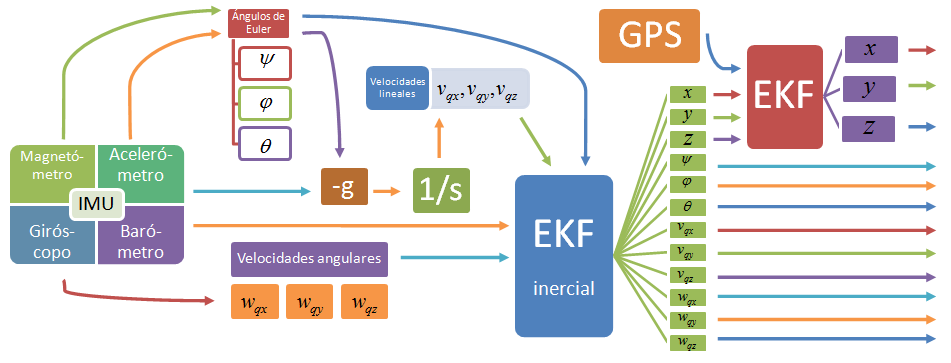
\includegraphics[width=1\textwidth]{./pics_kalman/diagrama_kalman.png}
	\caption{}
	\label{}
\end{figure}



\end{document}